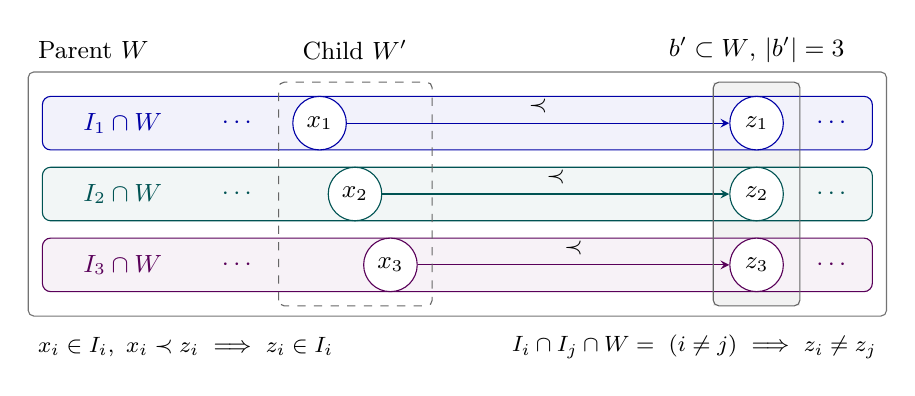
\begin{tikzpicture}[x=1cm,y=1cm,font=\small,>=stealth,
  job/.style={circle,draw,fill=white,minimum size=6.8mm,inner sep=0pt}]
  \draw[black!55,rounded corners=2pt] (-.15,-.25) rectangle (10.75,2.85);
  \node[anchor=west] at (-.15,3.13) {Parent $W$};
  \node at (4,3.13) {Child $W'$};
  \node at (9.1,3.13) {$b'\subset W$, $|b'|=3$};

  \fill[black!5] (8.55,-.12) rectangle (9.65,2.72);
  \foreach \yy/\ii/\xx/\cc in {2.2/1/3.55/blue!65!black,1.3/2/4/teal!65!black,.4/3/4.45/violet!70!black} {
    \draw[draw=\cc,fill=\cc!5,rounded corners=3pt]
      (.03,\yy-.34) rectangle (10.57,\yy+.34);
    \node[text=\cc] at (1.05,\yy) {$I_{\ii}\cap W$};
    \node[text=\cc] at (2.5,\yy) {$\cdots$};
    \node[job,draw=\cc] (x\ii) at (\xx,\yy) {$x_{\ii}$};
    \node[job,draw=\cc] (z\ii) at (9.1,\yy) {$z_{\ii}$};
    \draw[->,draw=\cc] (x\ii) -- node[above,font=\footnotesize] {$\prec$} (z\ii);
    \node[text=\cc] at (10.05,\yy) {$\cdots$};
  }
  \draw[dashed,black!60,rounded corners=2pt] (3.03,-.12) rectangle (4.98,2.72);
  \draw[black!60,rounded corners=2pt] (8.55,-.12) rectangle (9.65,2.72);
  \node[anchor=west,font=\footnotesize] at (-.15,-.64)
    {$x_i\in I_i,\ x_i\prec z_i\ \Longrightarrow\ z_i\in I_i$
     };
  \node[anchor=east,font=\footnotesize] at (10.75,-.64)
    {$I_i\cap I_j\cap W=\varnothing\ (i\ne j)\ \Longrightarrow\ z_i\ne z_j$};
\end{tikzpicture}
